\documentclass[12pt]{article}
\usepackage{tabularx} % extra features for tabular environment
\usepackage{amsmath}  % improve math presentation
\usepackage{graphicx} % takes care of graphic including machinery
\usepackage{amsthm}
\usepackage{amssymb}
\usepackage{bm}
\usepackage{bbm}
\usepackage{dsfont}
\usepackage{graphicx}
\usepackage{subfigure}
\usepackage[margin=1in]{geometry} % decreases margins
\usepackage{cite} % takes care of citations
%\usepackage{cleveref}
\usepackage[final]{hyperref} % adds hyper links inside the generated pdf file
\hypersetup{
	colorlinks=true,       % false: boxed links; true: colored links
	linkcolor=blue,        % color of internal links
	citecolor=blue,        % color of links to bibliography
	filecolor=magenta,     % color of file links
	urlcolor=blue         
}

%% Define a new 'leo' style for the package that will use a smaller font.
\makeatletter
\def\url@leostyle{%
	\@ifundefined{selectfont}{\def\UrlFont{\sf}}{\def\UrlFont{\small\ttfamily}}}
\makeatother
%% Now actually use the newly defined style.
\urlstyle{leo}
%\usepackage{cleveref}

%opening
\title{\textbf{STAT 605: Project Proposal}}
\author{\textbf{Kou Wang} \\ kwang432  \\ \and  \textbf{Shushu Zhang} \\ szhang695 \and \textbf{Xinyue Wang} \\ xwang2438 \and \textbf{Yiqun Xiao} \\ yxiao85 \and \textbf{Sixu Li} \\ sli739}
\date{}

\begin{document}
	\maketitle
	
\section{Introduction}
We are working on a subset of Amazon movie review data in this first draft, with 10000 observations and 10 variables. We are interested in \textit{mining which words have strong relationships to the five star rating and which ones highly correlate to the negative reviews.} Therefore, among the 10 variables, we mainly explore the relationship between user review texts and review scores. In achieving this goal, we first use some natural language processing (NLP) techniques, such as Document-Term Matrix (DTM) representation, TF-IDF to clean the data. Then, we use regularized lasso logistic regression to fit the model with cross-validation. We implement the code in R and run the code on CHTC. As a result, we select top 30 positive and negative words based on significance. 
 
\section{Statistical Analysis}
\label{sec:2}
%In this section, we provide detailed narratives of the process of data analysis. We first clean and extract useful information for the text data in \Cref{subsec:Cleaning}, and then use lasso to reduce the high dimension of the text data in \Cref{subsec:lasso}, and use regression to fit proper model in \Cref{subsec:mod}. 

\subsection{Data Description \& Data Cleaning}
\label{subsec:Cleaning}
The web data is provided by Jure Leskovec, an associate professor from Stanford University. It's a data set containing about 35 million reviews from Amazon. The corresponding time spans from June 1995 to March 2013, a period of 18 years. The size of whole data set is 11 gigabtyes and it is available on website \href{http://snap.stanford.edu/data/web-Amazon-links.html}{Amazon reviews}. In this first draft, we focus on the products of movie industry, and perform data analysis on a subset with 10000 reviews to try out before handling the whole data set. We mainly focus on user review texts and review scores (on a 1-5 scale).

In order to extract useful information from the reviews, we need to preprocess the text data using NLP techniques. We (1) transform the target reviews to corpus; (2) change to lower case; (3) remove all the numbers; (4) remove all the stop words; (5) strip whitespace;  (6) remove punctuation; (7) change to Document-Term Matrix (DTM) representation (i.e., reviews as rows, and words as columns, frequencies of the occurance of a word for each text review as values of the matrix); (8) remove sparse terms from a Term-Document Matrix with 0.99 threshold (i.e., remove all the words that occur less than 1\% of the number of the words) ; (9) use TF-IDF (Term Frequency-Inverse Document Frequency) to transform the matrix (with details filled below); (10) obtain binary response variable by replace all the review scores of 4,5 to 1, and 1,2,3 to 0; (11) use bigram frequencies; (12) split training and test data. 

Here are some details about TF-IDF. For DTM, if a word occurs more often than others in general, it is more likely to occur more frequently in a review, such as "movie" in our case, which is unfair to other words. Therefore, we use TF-IDF (Term Frequency-Inverse Document Frequency) to offset these effects. TF-IDF can be mathematically characterized by 
\begin{equation}
\begin{aligned}
TF(\omega,t)&=\frac{\mathrm{\#\omega~in~t}}{\mathrm{\#words~in~t}}\\
IDF(\omega,t)&=log(\frac{\mathrm{\#words~in~t}}{\mathrm{\#reviews~that~contains~\omega}})\\
TFIDF(\omega,t) &= TF(\omega,t)*IDF(\omega,t)
\end{aligned}
\end{equation}
where $\omega$ is a word and $t$ represents a review. 

\subsection{Statistical Models}

Lasso logistic regression is selected as the statistical model to apply on our document matrix. Since lasso procedure encourages simple and sparse models, we have reduced dimensions in the previous data preprocessing procedure. 

\subsubsection{Logistic Regression}

Logistic Regression is one of the few algorithms that is used for the task of Classification of data. Since we are interested in mining which words have strong relationships to the five star rating and which ones highly correlate to the negative reviews, and in regression analysis, the logistic regression  model is a form of binary regression and fits well in our purpose. In this project, logistic regression is estimating the parameters of a logistic model. Consider a generalized linear model function parameterized by $\theta$, 
$$
h_\theta(X)=\frac{1}{1+e^{-\theta^TX}}=Pr(Y=1|X;\theta)
$$
We are assuming that all the observations in the samples are independently Bernoulli distributed.

\subsubsection{Lasso}

Although we reduced our data dimension according to eliminate the sparsity, it is still not enough for our regression analysis due to the complexity of the natural language especially the meaning and the diversities of the variables. Lasso regression is a type of linear regression that uses shrinkage, which stands for least absolute shrinkage and selection operators. We decide to use the Lasso linear model function parameterization for our logistic regression. Lasso regression performs L1 regularization, which adds a penalty equal to the absolute value of the magnitude of coefficients. This kind of penalty fits well in our circumstances. Because this type of regularization can result in sparse model and the coefficients can be eliminated from the model. Larger penalties like L2 regularization (e.g. Ridge regression) can not result in elimination of coefficients or sparse models. By Lasso regression, we substantially reduced the number of variables.
$$
\hat{\beta}^\lambda = argmin_{\beta \in \mathbb{R}^p} ||y-X\beta||_2^2+\lambda||\beta||_1 \\
\hat{S}^\lambda = \{k:\hat{\beta}_k^\lambda \neq 0\}
$$
where $X \in\mathbb{R} ^{n*p} $ is the design matrix, $y \in \mathbb{R}^n$ is a vector of outputs, and $\lambda$ is a regularization parameter that controls the size of the selection set.

By implemented methods above with our training dataset provided by previous step, we fit our models and build our findings.

\subsection{Findings}

We finally found several word collocations associated with positive/negative review. Here is a image illustrating our findings. 

\begin{itemize}
	\item  story told, excellent job, along way, dog soldiers, fall love, highly recommend, well worth are associated with positive reviews
	\item needless say, two hours, sounds like, pretty bad, get wrong, waste money, bad movie, car chase, really wanted, seemed like, way much, new version, save money one worst are associated with negative reviews.
\end{itemize}

\begin{figure}
	\centering
	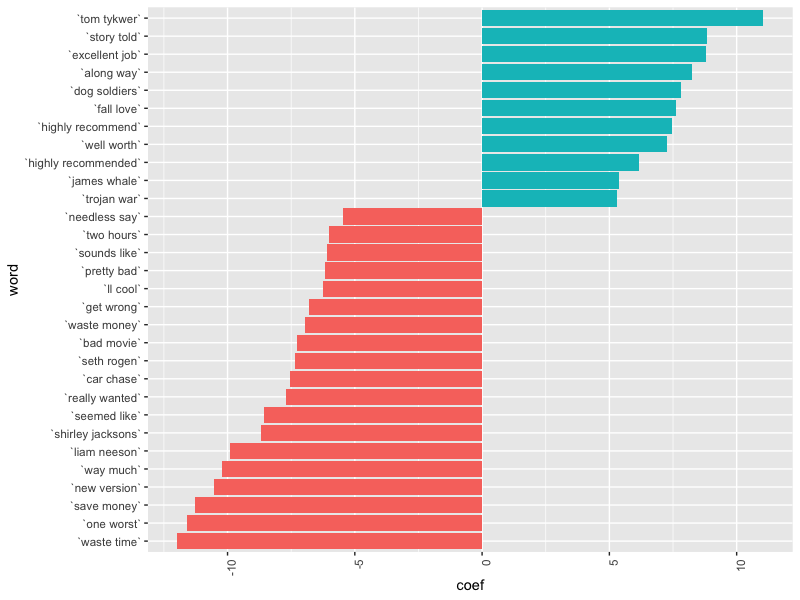
\includegraphics[scale=0.5]{../Image/Top_30_positive_and_negative_words.png}
	\caption{Top 30 positive and negative words}
	\label{fig:1}
\end{figure}

In figure \ref{fig:1}, we found that some words are seemed positive by ourselves but they are associated with negative reviews, which is interesting. And we also found some collocations do not make any sense. It may due to the process of using our corpus.



\section{Conclusion}
To draw our conclusion, in this project, a textual dataset with about 35 million reviews from Amazon  with a time span from June 1995 to March 2013 is analyzed. By cleaning the data and reducing the dimension, performing the DTM procedure, we obtained our word matrix as our explanatory matrix. We built two-word collocation as our variables and performing the lasso logistic regression, finally build our result: the words collection associated with positive/negative reviews. We found that some words are representing adverse attitude compared to our expectation. Further analyses need to be taken.



%\bibliographystyle{acm}
%\bibliography{ref}
\end{document}